\chapter{Návrh}
\label{kap:nav}
V tejto kapitole sa budeme zaoberať návrhom jednotlivých častí aplikácie. Najskôr spomenieme funkcie, ktoré bude naša aplikácia ponúkať. Ďalej popíšeme, ako sme spomedzi mnohých alternatív vybrali vhodný algoritmus pre potrebu našej aplikácie. Pri navrhovaní aplikácie sme sa venovali analýze získaných statických dát a dát o meškaní. Spomíname tiež, ako budeme pristupovať k týmto dátam pri implementácii, teda akým spôsobom ich uložíme do databázy a následne do dátovej štruktúry. V neposlednom rade spomenieme, ako bude fungovať naša aplikácia z pohľadu jej architektúry.

\section{Funkcie aplikácie}
Ako sme si mohli všimnúť v \ref{sec:applications}, všetky aplikácie ponúkajú vyhľadávanie z aktuálnej polohy rovnako, ako aj možnosť výberu zastávky priamo z mapy. Tieto funkcie bude používateľovi ponúkať aj naša aplikácia. Väčšina spomenutých aplikácií ponúkala zobrazenie histórie vyhľadávania, ktorá odľahčí používateľa od zadávania parametrov v prípade, že vyhľadáva väčšinou tie isté spoje. Túto funkcionalitu nájde používateľ aj v našej aplikácii. História vyhľadávania sa bude ukladať do pamäte zariadenia. 

Okrem aplikácie \textit{UBIAN} a \textit{CP} si používatelia vedia zobraziť všetky linky v MHD a postupnosti zastávok, ktoré obsluhujú. Túto funkciu bude ponúkať aj naša aplikácia. Čo sa týka nastavenia prídavných preferencií pri vyhľadávaní, aplikácie ponúkajú rôzne preferencie. Najčastejšími z nich sú: maximálny počet prestupov, minimálny čas na prestup, limit pre peší presun a zobrazenie len nízkopodlažých vozidiel. Naša aplikácia bude mať možnosť nastavenia všetkých týchto preferencií.

Jediná aplikácia, ktorá ponúka informácie o reálnom pohybe vozidiel vo forme meškania, je aplikácia \textit{UBIAN}. Predpokladáme však, že aj táto aplikácia vyhľadáva v statických cestovných poriadkoch a pri vyhľadanom spoji len pripíše informáciu vo forme meškania. Uvažujeme tak na základe toho, že po vyhľadaní spojov zo zastávky po zadaní aktuálneho času aplikácia ponúkne také spoje, ktoré podľa statických cestovných poriadkov majú na túto zastávku v blízkej budúcnosti príchod. Ak existuje taký spoj, ktorý mal odchod z danej zastávky v minulosti, ale má meškanie a na zastávke ešte nebol, aplikácia ho nezobrazí. Naša aplikácia ponúkne aj tie spojenia, ktoré kvôli meškaniu na zastávku ešte nedorazili. Pre vyhľadaný spoj zobrazí čas odchodu zo statických dát cestovného poriadku a pripíše k nemu informáciu o meškaní.

Medzi ďalšie funkcionality patrí zakúpenie lístka priamo cez aplikáciu. Táto funkcionalita však nesúvisí priamo so zadaním našej práce a navyše je potrebná zmluva s dopravcami. Preto naša aplikácia túto možnosť ponúkať nebude.

Len aplikácia \textit{CG Tranzit} funguje aj v offline režime. Hoci je užitočné ponúknuť vyhľadávanie bez možnosti prístupu na internet, znamenalo by to, že náš algoritmus by bežal na klientskej strane.  Keďže hlavnou úlohou našej aplikácie je vyhľadávanie spojov z reálnych dát, aplikácia bude fungovať online s tým, že zaručí používateľom vždy aktuálne spojenia. 

V tabuľke \ref{table:aplication-funcions} je zobrazený prehľad funkcionalít našej navrhovanej aplikácie a iných existujúcich aplikácii na vyhľadávanie spojov v MHD Bratislava.

\begin{table}[H]
\footnotesize
\begin{tabular}{|L{4.49cm}|c|c|c|C{1.29cm}|c|C{1.54cm}|}
\hline
\rowcolor[HTML]{C0C0C0} 
\textbf{} & \textbf{Imhd.sk} & \textbf{IDS BK} & \textbf{CP} & \textbf{CG Tranzit} & \textbf{UBIAN} & \textbf{Naša aplikácia}
\\ \hline
\textbf{z aktuálnej polohy} & \cmark & \cmark  & \cmark  & \cmark  & \cmark  & \cmark    
\\ \hline
\textbf{výber zástavok z mapy} & \cmark & \cmark  & \cmark  & \cmark  & \cmark & \cmark       
\\ \hline
\textbf{história vyhľadávania} & \cmark & \xmark  & \cmark  & \cmark  & \cmark & \cmark         
\\ \hline
\textbf{zobrazenie liniek} & \cmark & \cmark  & \xmark  & \cmark  & \xmark & \cmark         
\\ \hline
\textbf{max. počet prestupov} & \cmark & \cmark  & \cmark  & \cmark  & \xmark & \cmark         
\\ \hline
\textbf{min. čas na prestup} & \cmark & \xmark  & \cmark  & \cmark  & \xmark & \cmark         
\\ \hline
\textbf{limit pre peší presun} & \cmark & \cmark  & \xmark  & \xmark  & \xmark  & \cmark        
\\ \hline
\textbf{len nízkopodlažné vozidlá} & \cmark & \xmark  & \cmark  & \xmark  & \xmark  & \cmark        
\\ \hline
\textbf{meškanie MHD} & \xmark & \xmark  & \xmark  & \xmark  & \cmark & \cmark         
\\ \hline
\textbf{kúpa lístkov} & \xmark & \cmark  & \cmark  & \cmark  & \cmark & \xmark         
\\ \hline
\textbf{offline režim} & \xmark & \xmark  & \xmark  & \cmark  & \xmark  & \xmark        
\\ \hline
\end{tabular}
\caption{Tabuľka funkcionalít existujúcich aplikácií a navrhovanej aplikácie}
\label{table:aplication-funcions}
\end{table}

\section{Algoritmus}
Pri hľadaní algoritmu na nájdenie optimálnej cesty sme najskôr siahli po najznámejšom vyhľadávacom grafovom algoritme. Dijkstrov algoritmus \ref{sec:dijkstra} sa zdal vhodný, avšak jeho vylepšená verzia A* algoritmus \ref{sec:a-star} je pri správne zvolenej heuristike efektívnejšia. Keďže zastávky, ktoré predstavujú vrcholy v grafe majú dané súradnice, môžeme pri vyhľadávaní optimalizovať prehľadávaný priestor. Pri štúdiu článkov sme narazili na rôzne optimalizácie prehľadávaného priestoru. Minimalizácia v okolí virtuálnej cesty a minimalizácia \textit{bounding boxom} sú spomenuté v \ref{sec:optimalization}.

V prípade cestovných poriadkov je náročné správne namodelovať graf, ktorý dokáže efektívne spracovať časovo závislé dáta. V \ref{sec:models} boli spomenuté dva overené prístupy \textit{Time dependent} a \textit{Time expanded model}, ktoré tento problém riešia. 

Ďalšou výzvou je prispôsobiť grafový vyhľadávací algoritmus, aby dokázal vypočítať najoptimálnejšiu cestu, prihliadal na prestupy medzi rôznymi módmi a popri tom počítal s ďalšími pridanými kritériami.
V \ref{sec:time-dependant-algorithm} boli spomenuté návrhy časovo závislých algoritmov. Algoritmus \ref{sec:multimodal-algorithm} sa dokáže vysporiadať aj viacerými módmi. Vráti však len jednu cestu. V \ref{sec:alternative-optimal-paths} je popísaný algoritmus, ktorý efektívne vyhľadáva rôzne alternatívne cesty.

Kvôli dynamickej povahe verejnej dopravy grafový prístup v kombinácii s vyhľadávacím grafovým algoritmom vyžaduje veľa pre-processingu a to sa odráža na výpočtových časoch. Výhodou vo verejnej doprave je, že vozidlá sa pohybujú po vyznačených linkách, ktorých trasy poznáme. Schéma verejnej dopravy sa preto dá zachytiť do pomerne jednoduchých dátových štruktúr. Tento fakt si všimli aj autori algoritmu RAPTOR, ktorý sme opísali v \ref{sec:raptor}. 

V našej aplikácii sme sa rozhodli použiť tento negrafový algoritmus.
Jeho výhodou je, že nie je potrebné vytvárať model a nie je potrebné riešiť multimodalitu hromadnej dopravy. Ľahšie zvláda dynamickosť dát ako meškanie linky, zrušenie linky alebo zmenu trasy. 

Využijeme základnú verziu RAPTOR algoritmu popísanú v \ref{sub:raptor-basic} a súčasne využijeme aj jeho optimalizáciu opísanú v \ref{sub:raptor-optimalisation}, kedy označujeme zastávky, aby sme nemuseli prechádzať tie linky, ktorým sa nevylepšil čas $\tau_{k-1}(p)$. Optimalizáciu \textit{local-prunning} nevyužijeme, keďže chceme použiť rozšírenú verziu RAPTOR algoritmu a to je rRAPTOR algoritmus popísaný v sekcii \ref{sub:rraptor}. Algoritmus rRAPTOR nám nevráti len jednu najkratšiu cestu, ktorá začína najskôr od zadaného času, ale vráti nám množinu najkratších ciest, začínajúcich v zadanom časovom úseku.

Cesta, ktorú nám vráti základná verzia RAPTOR algoritmu je najkratšia a nezáleží na tom, koľko prestupov bude obsahovať. Našou úlohou je používateľovi poskytnúť optimálnu cestu a keďže optimálna cesta môže byť pre každého používateľa iná, ponúkneme mu viacero alternatív.  Túto funkciu ponúka vylepšený RAPTOR algoritmus popísaný v \ref{sec:raptor-improved}. Algoritmus nám vráti viacero optimálnych ciest, pričom prihliada na to, aby jednotlivé cesty neboli rovnaké na veľkej časti úseku.

Našim cieľom je zlúčiť rRAPTOR algoritmus s vylepšeným RAPTOR algoritmom na hľadanie viacerých ciest a zakomponovať mechanizmus schopný zohľadniť zadané používateľské preferencie, ktoré bude algoritmus prijímať ako vstupné parametre. Preferencie, ktoré bude vedieť algoritmus zohľadniť: minimálny čas na prestup, maximálny počet prestupov, maximálna dĺžka pešieho prestupu a vyhľadanie len nízkopodlažných spojov. Na obrázku \ref{fig:algorithm} sú zachytené jednotlivé podalgoritmy, ktoré budú tvoriť náš výsledný algoritmus.

\begin{figure}[H]
\centerline{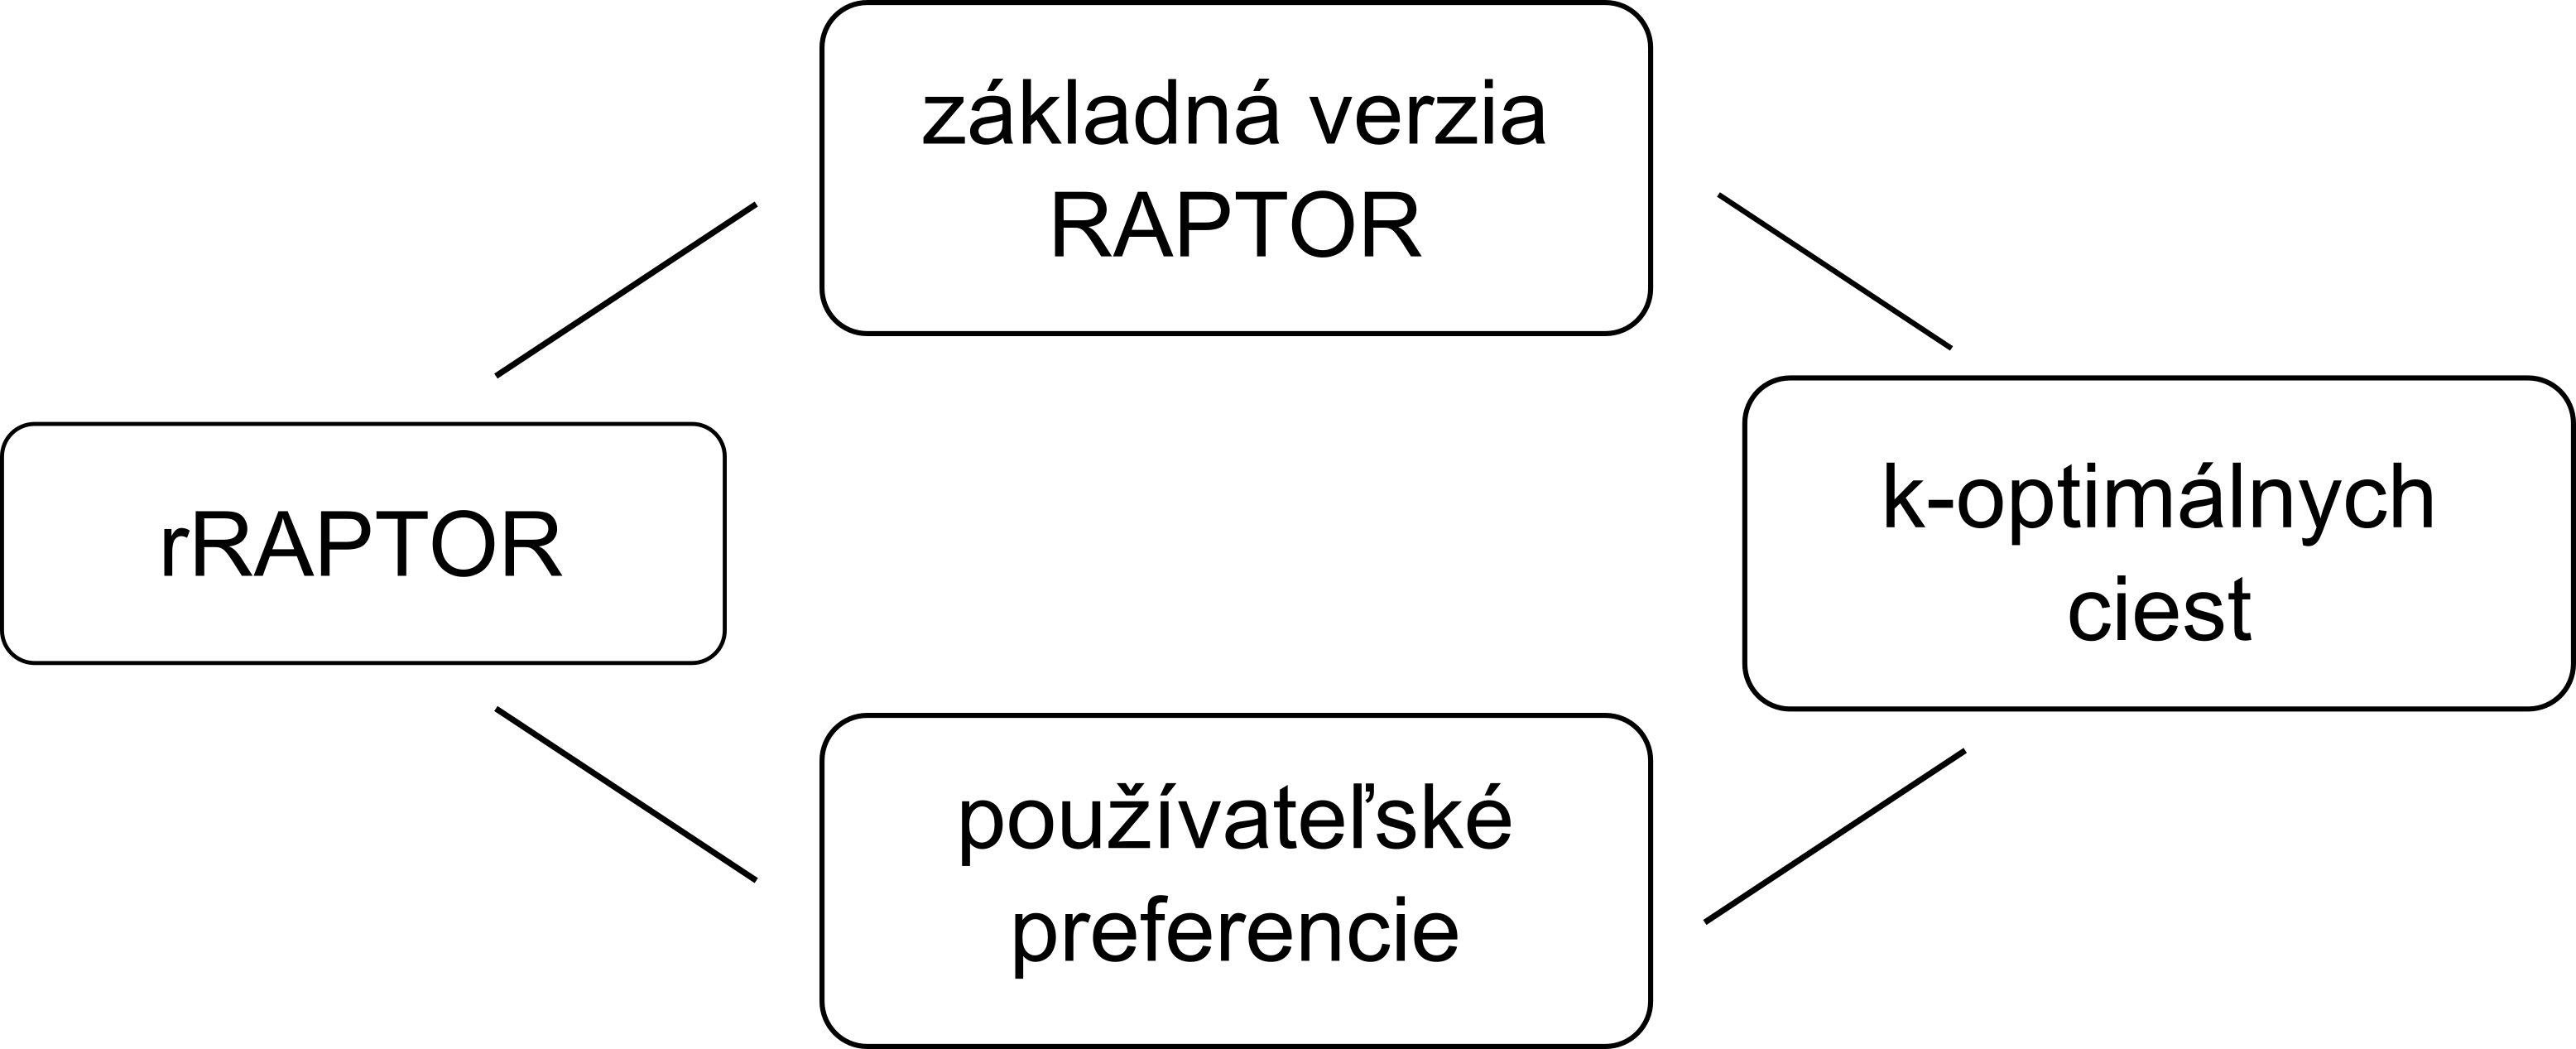
\includegraphics[width=0.8\textwidth]{images/algorithm}}
\caption[Návrh algoritmu]{Návrh algoritmu}
\label{fig:algorithm}
\end{figure}

Výstupom z nášho algoritmu bude množina ciest začínajúcich na zastávke $p_s$, po čase $\tau$ a končiacich v zastávke $p_t$. Jednotlivé cesty sú optimálne, vyhovujú prípadným používateľským preferenciám a ich časy odchodov sú z časového intervalu <$\tau, \tau + \Delta \tau$>. 

\subsection{Vyhľadávanie z aktuálnej polohy}
Ak používateľ zadá ako začiatočnú zastávku aktuálnu polohu, nájdeme zastávky v okolí radiálnym vyhľadávaním, ako bolo spomenuté v \ref{sec:actual-location}. Najbližšia vyhľadaná zastávka k aktuálnemu bodu nemusí znamenať optimálne riešenie a preto budeme považovať za začiatočnú zastávku každú z nich. Pre každú zastávku zvlášť spustíme algoritmus, ktorý nám pre každú zo zastávok vráti množinu optimálnych ciest a na záver z nich vyberieme $n$ najoptimálnejších ciest. Do finálneho riešenia zakomponujeme peší presun od aktuálnej polohy po začiatočnú zastávku vybraných optimálnych ciest.

\section{Dáta}
Pri vývoji aplikácie a pre jej testovanie sú nevyhnutné dáta. Pre účely aplikácie budeme potrebovať dáta zo statických cestovných poriadkov a dáta o meškaní jednotlivých jázd. 

\subsection{Dáta statických cestovných poriadkov}
Od Dopravného podniku Bratislava sme získali statické cestovné poriadky, ktoré mali platnosť od $5.2.2018$ – $31.12.2018$. Dáta sú vo formáte GTFS. 

\subsubsection{GTFS}

\subsection{Dáta o meškaní}
Podarilo sa nám získať aj informácie o meškaní za rok 2018, pre mesiac február, marec a apríl. Pre každý deň v mesiaci existuje súbor vo formáte .csv. Každý záznam obsahuje údaje:
\begin{itemize}
\item{Id – identifikačné číslo záznamu}
\item{Datum a cas – dátum a čas, kedy bol záznam o meškaní zaevidovaný}
\item{Vozidlo – identifikačné číslo vozidla}
\item{Linka – identifikačné číslo linky}
\item{Poradie – poradie jazdy v linke}
\item{Cislo zastavky – identifikačné číslo zastávky}
\item{Nazov zastavky – názov zastávky}
\item{Meskanie – hodnota meškania v minútach.}
\end{itemize}

Z pozorovania dát vyplýva, že hodnoty meškania majú hodnotu $0$, záporné celé čísla alebo hodnotu $n/a$. V prípade, že narazíme na hodnotu $0$ alebo $n/a$, tento záznam neberieme do úvahy. Môže ale platiť, že hodnota $0$ znamená, že meškanie je z intervalu $<0 min, 1 min)$ minúta, hodnota $1$ z intervalu $<1 min, 2 min)$. Na prelome dní sa tam vyskytuje hodnota $-1229$. 

Takže naša aplikácia bude môcť ponúknuť správne cesty s prihliadnutím na meškanie spojov od $5.2.2018$ – $30.4.2018$. Statické vyhľadávanie bez meškania bude správne fungovať od $5.2.2018$ do konca roka $2018$.

\subsection{Pešie presuny}
V dátach sa nenachádzajú informácie o peších presunoch. \textit{Google API} ponúka možnosť vyhľadania peších vzdialeností medzi 2 bodmi. Počet bezplatných dopytov na \textit{Distance Matrix API} je obmedzený. Nebudeme vyhľadávať pešie vzdialenosti medzi každou dvojicou zastávok, nakoľko je to nepotrebné. 
Budeme postupovať nasledovne: pre každú zastávku $p$ nájdeme zastávky v okolí 800 metrov radiálnym vyhľadávaním. Pomocou \textit{Distance Matrix API} zistím vzdialenosti nájdených zastávok od zastávky $p$. Každú dvojicu zastávok uložíme do súboru \textit{foot\_paths.txt} spolu so zistenými vzdialenosťami určených v minútach.


\section{Databáza}

Na serveri budú uložené dáta aplikácie v PostgreSQL databáze. Databáza sa naplní pri prvotnom spustení aplikácie na serveri. Schéma databázy je popísaná entitno-relačným diagramom na obrázku \ref{fig:erd}.

\begin{figure}[H]
\centerline{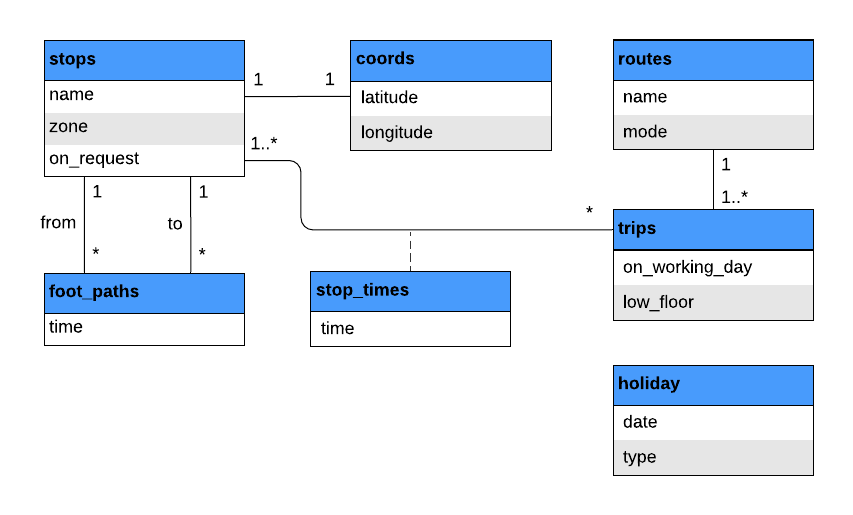
\includegraphics[width=1.0\textwidth]{images/ERD}}
\caption[Entitno-relačný diagram]{Entitno-relačný diagram}
\label{fig:erd}
\end{figure}

Entita \textit{stop\_areas} obsahuje zoskupenie zastávok, ktoré majú rovnaké názvy (\textit{name}). 


V entite \textit{stops} evidujeme zónu mesta (\textit{zone}), do ktorej zastávka patrí. Hodnotu \textit{on\_request}, určuje, či sa na  zastávke nastupuje a vystupuje na znamenie. Každá zastávka má priradené súradnice, ktoré sa udržujú v entite \textit{coords}.

V entite \textit{coords} sú súradnice určené atribútmi zemepisná šírka (\textit{latitude}) a zemepisná výška (\textit{longitude}). 

Entita \textit{foot\_paths} obsahuje atribút \textit{time}, ktorý určuje čas v minútach potrebný na peší presun zo zastávky \textit{from} na zastávku \textit{to}.

V entite \textit{routes} sa udržuje zoznam liniek jazdiacich aktuálne v bratislavskej MHD. Linka je určená názvom (\textit{name}) a módom (\textit{mode}). V Bratislave jazdia 3 rôzne módy: električka, trolejbus a autobus. Každá linka má počas dňa viaceré jazdy (\textit{trips}).

Entita (\textit{trips}) uchováva informáciu o tom, či je vozidlo, ktoré bolo pridelené konkrétnej jazde nízkopodlažné (\textit{low\_floor}), ktorým smerom ide (\textit{direction}) a zároveň počas akých typov dní (\textit{service\_day}) jazda premáva. Každá jazda linky je tvorená postupnosťou zastávok, ktoré linka obsluhuje.

V entite \textit{stop\_times} je zachytený čas (\textit{time}), kedy jazda stojá na zastávke a v akom poradí sú zastávky v rámci jazdy (\textit{sequence\_order}).

V entite \textit{service\_days} sú názvy rôznych typov dní, v ktorých premávajú jazdy liniek. 

Entita \textit{calendar\_dates} obsahuje zoznam všetkých dátumov (\textit{date}), v rozsahu platnosti aktuálneho cestovného poriadku. Ku každému dátumu je priradený typ dňa (\textit{service\_day}). Jeden dátum môže prislúchať k viacerým typom dňa a naopak jeden typ dňa môže prislúchať viacerým dátumom.

\section{Dátová štruktúra}
Rovnako dôležit8 je dobre navrhnutá dátová štruktúra, s ktorou bude algoritmus vedieť rýchlo a efektívne pracovať. Budeme sa inšpirovať dátovou štruktúrou z \ref{subsec:structure}, ktorá bola navrhnutá pre základnú verziu RAPTOR algoritmu. Dátová štruktúra bude obsahovať aktuálne cestovné poriadky s prispôsobenými príchodmi a odchodmi vozidiel podľa prípadných meškaní.  

Dátová štruktúra uvedená v článku ráta s tým, že jednotlivé jazdy v rámci linky majú rovnakú postupnosť zastávok. V našich dátach to tak nie je. Linka obsahuje jazdy, ktoré idú jedným aj druhým smerom. Zástavky cez ktoré prechádza linka majú síce rovnaký názov, ale majú iné identifikačné čísla, ktorými sú definované. Okrem rôznych smerov obsahuje linka aj také jazdy, ktorých postupnosť zastávok je iná ako pri väčšine. Najmä v ranných a večerných hodinách prechádzajú niektoré jazdy len cez určitú podpostupnosť zastávok. 
RAPTOR algoritmus potrebuje, aby všetky jazdy, ktoré patria konkrétnej linke mali rovnakú postupnosť zastávok. Rozhodli sme sa preto zoskupiť jazdy s rovnakou postupnosťou zastávok do úsekov. Teraz platí, že 1 linka má viacero úsekov a jednému úseku linky prislúcha viac jázd linky. 

Často sa potrebujeme dopytovať na všetky linky, ktoré stoja na konkrétnej zastávke a rovnako potrebujem vedieť postupnosť zastávok, ktoré patria konkrétnej linke. 

\textit{StopTimes} bude objekt alebo pole, ktoré obsahuje nielen informáciu o čase, kedy podľa statického poriadku má stáť jazda linky na zastávke, ale aj informáciu o predpokladanom časovom meškaní danej jazdy na zastávku.


\section{Architektúra aplikácie}

Klient sa bude dopytovať na server pre vyhľadanie spojenia. Server spustí výpočet nad dátovou štruktúrou, ktorá má aktuálne cestovné poriadky s imformáciou o prípadnom meškaní spojov a vráti odpoveď klientovi.

Algoritmus bude pracovať nad dátovou štruktúrou, ktorá bude obsahovať stále aktuálne dáta. Dátová štruktúra bude rovnako ako algoritmus uložená na serverovej strane. 

\subsection{Serverová strana}
Na serverovej strane bude bežať aplikačný server \textit{Tomcat}. Na uchovanie dát použijeme relačnú databázu. Na komunikáciu s klientom budeme používať \textit{REST API}.

\subsection{Klientská strana}
Na klientskej strane sme sa rozhodli pre progresívnu webovú aplikáciu \textit{PWA}. Je to webová aplikácia, ktorá sa dokáže správať ako mobilná aplikácia, neustále sa aktualizuje, pričom nie je potrebná jej inštalácia. Po návšteve webovej stránky na mobilnom zariadení používateľ dostane upozornenie od stránky, či si ju chce uložiť do zariadenia ako mobilnú aplikáciu. Progresívna webová aplikácia zaberá minimum miesta v pamäti a má svoj vlastný úložný priestor, kde sa budú ukladať preferencie a história vyhľadávania.

\subsection{Spracovanie dát}
Pri spustení aplikácie alebo po aktualizácii cestovných poriadkov sa spustí služba, ktorá nám z úložiska, kde sú aktuálne cestovné poriadky namapuje dáta do našej databázy. Po tom, ako budú dáta uložené v databáze sa spustí ďalšia služba, ktorá obnoví dátovú štruktúru podľa nových cestovných poriadkov. 

Ďalšia služba bude vytvorená na spracovanie údajov o meškaní. Hoci máme v súbore pre konkrétny deň údaje o meškaní jázd na celý deň, chceme sa čo najviac priblížiť reálnemu nasadeniu. Budeme teda rátať s tým, že nové údaje o meškaní pribúdajú po minúte. Služba bude spúšťaná každú minútu. Bude čítať súbor pre aktuálny deň, získa záznamy, ktoré pribudli v poslednej minúte a aktualizuje meškanie pre konkrétnu jazdu. Údaje o meškaní sú evidované pre zastávku s, na ktorej meškanie vzniklo. Aktualizácia meškania jazdy bude prebiehať tak, že pre všetky zastávky jazdy od zastávky s až po konečnú zastávku jazdy zapíše do dátovej štruktúry hodnotu získaného meškania.

Spôsob akým bude aplikácia nasadená je znázornená na obrázku \ref{fig:deploymentDiagram}.

\begin{figure}[H]
\centerline{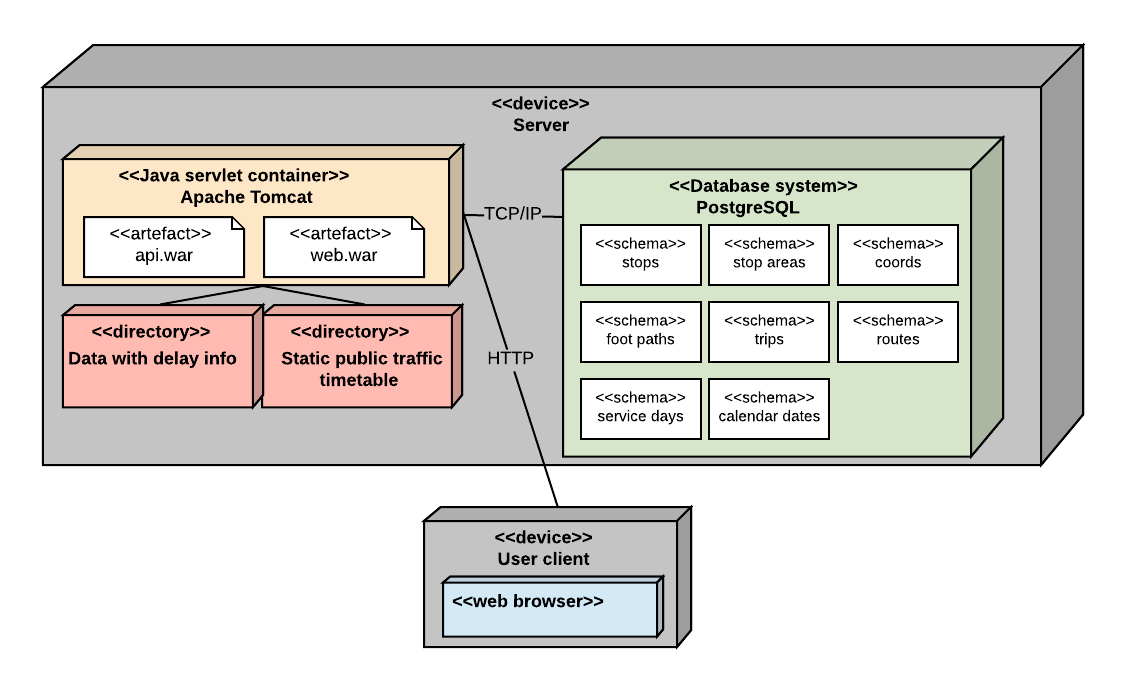
\includegraphics[width=1.0\textwidth]{images/deployment-diagram}}
\caption[Diagram nasadenia]{Diagram nasadenia)}
\label{fig:deploymentDiagram}
\end{figure}



